\documentclass[letterpaper, 10 pt, conference]{ieeeconf}
\IEEEoverridecommandlockouts
\overrideIEEEmargins
\pdfminorversion=4
\input{./sections/pre_document.tex}

\begin{document}

\title{\LARGE \bf Scan-matching of panoramic 2D range scans}


\author{Alexandros Filotheou, Andreas L. Symeonidis, Georgios D. Sergiadis, Antonis G. Dimitriou% <-this % stops a space
  \thanks{This work was supported by the European Union and Greek National Funds
  through the Operational Program Competitiveness, Entrepreneurship, and
  Innovation, under the call Research Create Innovate under Project T2EDK-02000.
  Corresponding author: Alexandros Filotheou, {\tt\small alefilot@auth.gr}.
  The authors are with the Department of Electrical and Computer Engineering,
  Aristotle University of Thessaloniki, 54124 Thessaloniki, Greece}
}

\maketitle
\thispagestyle{empty}
\pagestyle{empty}


%%%%%%%%%%%%%%%%%%%%%%%%%%%%%%%%%%%%%%%%%%%%%%%%%%%%%%%%%%%%%%%%%%%%%%%%%%%%%%%%
\begin{abstract}
  A real-time method for matching 2D range scans extracted from a LIDAR sensor
whose field of view is $2\pi$ is proposed. The method leverages properties of
the Fourier transform which arise due to the periodicity of the range signal.
The solution to scan-matching is given by transforming the problem into a
scan--to--map-scan matching problem. Matching is performed in a
correspondenceless manner. The proposed method outperforms established
scan-matching methods in terms of pose accuracy and robustness in tests on
public domain data and over sensor noise levels of commercially available range
sensors. The source code is available for download.

\end{abstract}

\begin{keywords}
Scan-matching, localisation, panoramic LIDAR
\end{keywords}

%%%%%%%%%%%%%%%%%%%%%%%%%%%%%%%%%%%%%%%%%%%%%%%%%%%%%%%%%%%%%%%%%%%%%%%%%%%%%%%%
\section{Introduction}
  
Contribution: invariant to large angular errors


%%%%%%%%%%%%%%%%%%%%%%%%%%%%%%%%%%%%%%%%%%%%%%%%%%%%%%%%%%%%%%%%%%%%%%%%%%%%%%%%
\section{Definitions}
  \label{section:definitions}
  %%%%%%%%%%%%%%%%%%%%%%%%%%%%%%%%%%%%%%%%%%%%%%%%%%%%%%%%%%%%%%%%%%%%%%%%%%%%%%%%
\begin{definition}
  \label{def:definition_1}
  \textit{Definition of a range scan captured from a conventional 2D LIDAR
  sensor.} A conventional 2D LIDAR sensor provides a finite number of ranges,
  i.e. distances to objects within its range, on a horizontal cross-section of
  its environment, at regular angular and temporal intervals, over a defined
  angular range \cite{lidar}. A range scan $\mathcal{S}$, consisting
  of $N_s$ rays over an angular range $\lambda$, is an ordered map
  $\mathcal{S} : \Theta \rightarrow \mathbb{R}_{\geq 0}$, $\Theta =
  \{\theta_n \in [-\frac{\lambda}{2}, +\frac{\lambda}{2}) : \theta_n =
  -\frac{\lambda}{2} + \lambda \frac{n}{N_s}$, $n = 0,1,\dots, N_s$$-$$1$$\}$.
  Angles $\theta_n$ are expressed relative to the sensor's heading, in the
  sensor's frame of reference. The angular distance between two consecutive
  rays is the sensor's angle increment $\gamma \triangleq \lambda/N_s$.
\end{definition}

%%%%%%%%%%%%%%%%%%%%%%%%%%%%%%%%%%%%%%%%%%%%%%%%%%%%%%%%%%%%%%%%%%%%%%%%%%%%%%%%
%\begin{definition}
  %\label{def:definition_2}
  %\textit{Scan-matching (or scan-to-scan matching) using a 2D LIDAR sensor} (adapted for use in
  %two dimensions from \cite{plicp}).
  %Let two range scans as defined by Definition \ref{def:definition_1},
  %$\mathcal{S}_R$ and $\mathcal{S}_V$, be captured from a LIDAR
  %sensor operating in the same environment at both capturing times. Let
  %$\bm{p}_V(x_V,y_V,\theta_V)$ be the pose from
  %which the sensor captured $\mathcal{S}_V$, expressed in some coordinate
  %system (usually a past pose estimate of the sensor). The objective of
  %scan-matching in two dimensions is to find the roto-translation
  %$\bm{q} = (\bm{t}, \theta)$, $\bm{t} = (\Delta x, \Delta y)$ that minimises
  %the distance of the endpoints of $\mathcal{S}_V$ roto-translated by
  %$\bm{q}$ to their projection on $\mathcal{S}_R$. Denoting the
  %endpoints of $\mathcal{S}_V$ by $\{\bm{p}_V^i\}$, in formula:
  %\begin{align}
    %\underset{\bm{q}}{\min} \sum\limits_i \Big\| \bm{p}_V^i \oplus \bm{q} - \prod \{ \mathcal{S}_R, \bm{p}_V^i \oplus \bm{q} \}\Big\|^2
    %\label{eq:s2sm_def}
  %\end{align}
  %The symbol ``$\oplus$" denotes the roto-translation operator
  %$\bm{p}_V^i \oplus (\bm{t}, \theta) \triangleq \bm{R}(\theta) \bm{p}^i_V + \bm{t}$,
  %where $\bm{R}(\theta)$ is the 2D rotation matrix for argument angle $\theta$,
  %and $\prod\{\mathcal{S}_R, \bm{p}_V^i \oplus \bm{q} \}$ denotes
  %the Euclidean projector on $\mathcal{S}_R$.
%\end{definition}


%%%%%%%%%%%%%%%%%%%%%%%%%%%%%%%%%%%%%%%%%%%%%%%%%%%%%%%%%%%%%%%%%%%%%%%%%%%%%%%%
\begin{definition}
  \label{def:definition_3}
  \textit{Definition of a map-scan.}
  A map-scan is a virtual scan that encapsulates the same pieces of information
  as a scan derived from a physical sensor. Only their underlying operating
  principle is different due to the fact the map-scan refers to distances to
  the boundaries of a point-set, referred to as the map, rather than within a
  real environment. A map-scan is derived by means of locating intersections of
  rays emanating from the estimate of the sensor's pose estimate and the
  boundaries of the map.
\end{definition}


%%%%%%%%%%%%%%%%%%%%%%%%%%%%%%%%%%%%%%%%%%%%%%%%%%%%%%%%%%%%%%%%%%%%%%%%%%%%%%%%
\section{Problem Formulation}
  \label{section:the_problem}
  \begin{problem}
  \label{prob:the_problem}
  Let a mobile robot, capable of motion in the $x-y$ plane, be equipped with a
  coplanarly mounted range scan sensor emitting $N_s$ rays. Let
  also the following be available or standing:
  \begin{itemize}
    \item The angular range of the range sensor is $360^\circ$
    \item A 2D range scan $\mathcal{S}_0$, captured at time $t_0$
    \item A 2D range scan $\mathcal{S}_1$, captured at $t_1 \geq t_0$
  \end{itemize}
\end{problem}
Then the objective is estimating the 3D rigid-body transformation
$\bm{T} = (\Delta x, \Delta y, \Delta \theta)$ which, when applied to the
endpoints of $\mathcal{S}_1$, aligns them to those of $\mathcal{S}_0$ with the
least error. Equivalently, roto-translation $\bm{T}$ corresponds to the
relative motion of the sensor from the pose where it captured $\mathcal{S}_0$
to the pose from which it captured $\mathcal{S}_1$.


%%%%%%%%%%%%%%%%%%%%%%%%%%%%%%%%%%%%%%%%%%%%%%%%%%%%%%%%%%%%%%%%%%%%%%%%%%%%%%%%
\section{Prior Work}
  \label{section:sota}
  Scan-matching with the use of a 2D LIDAR sensor began with IDC \cite{LuMilios},
an algorithm incorporating elements of the Iterative Closest Point (ICP)
algorithm \cite{ICP}. The latter and its variants, e.g.
\cite{weighted}-\cite{plicp}, have become the de facto scan-matching algorithms
in 2D and 3D settings, and research using ICP is still ongoing
\cite{ICP_var_1}-\cite{Marchel}. In particular, PL-ICP \cite{plicp} has been
widely adopted due to its increased accuracy among ICP variants, and the
availability of its source code. ICP and its variants, however, exhibit varying
performance \cite{icp_comp_trade}, limited by the noise level in the input
scans, the choice of prior, and the configuration of the parameters
governing their response. For these reasons, as well as for reasons of
robustness, the method of establishing correspondences shifted from
point-to-point or point-to-line to feature-to-feature. Commonly appearing
features for recognition are line segments \cite{CLS}\cite{Haytham}\cite{Wen},
SIFT features \cite{Jiayuan}, or features extracted through the use of deep
learning techniques \cite{Jiaxin}. In parallel, and for reasons of
indepencency from chance features or tailoring methods to specific
circumstances, research sprung around methods that extract or exploit
mathematical properties from range scans, or that view the problem of
scan-matching as an optimisation problem. Examples include correlation-based
methods \cite{olson},\cite{olson_2015}-\cite{Konecny}, feature distribution
matching \cite{HSM}, or matching by cost function minimisation \cite{PB_PSM}.



%%%%%%%%%%%%%%%%%%%%%%%%%%%%%%%%%%%%%%%%%%%%%%%%%%%%%%%%%%%%%%%%%%%%%%%%%%%%%%%%
\section{Approach}
  \label{section:the_proposed_method}
  The panoramic 2D scan-matching problem is iteratively decomposed into two
disjunctive sub-problems. The first is estimating the relative orientation of
$\mathcal{S}_1$ with respect to $\mathcal{S}_0$ under the assumption that both
are captured from the same location. The second is estimating the relative
displacement of $\mathcal{S}_1$ with respect to $\mathcal{S}_0$ under the
assumption that both are captured from poses of the same orientation. Solving
the first sub-problem is followed by the solution to the second sub-problem.
This process is iterated until termination conditions are met.

The orientation and location estimation submethods are presented in subsections
\ref{subsec:method_orientation_correction} and
\ref{subsec:method_location_correction} respectively. Subsection
\ref{subsec:method_pose_correction} presents the method of how these two
are woven together into the system that solves Problem \ref{prob:the_problem}
that is proposed in this work.

\subsection{Estimation of Relative Orientation}
  \label{subsec:method_orientation_correction}
  Let the assumptions of Problem \ref{prob:the_problem} be standing. Assume that
the two scans were captured from the same location but from different
orientations. Denoting with $\mathcal{F}\{\mathcal{S}\}$ the Discrete Fourier
Transform of signal $\mathcal{S}$, with $\mathcal{F}^{-1}\{\mathcal{S}\}$
its inverse, with $\bm{c}^\ast$ the conjugate of complex $\bm{c}$, and with
$|\bm{c}|$ its magnitude, calculate
$Q_{\mathcal{S}_0, \mathcal{S}_1}$:
\begin{align}
  Q_{\mathcal{S}_0, \mathcal{S}_1} \triangleq \dfrac{\mathcal{F}\{\mathcal{S}_0\}^{\ast} \cdot \mathcal{F}\{\mathcal{S}_1\}}{|\mathcal{F}\{\mathcal{S}_0\}| \cdot |\mathcal{F}\{\mathcal{S}_1\}|}
\end{align}
on the basis that if space is sampled sufficiently densely, for
$k,\xi \in \mathbb{Z}$: $k,\xi \in [0, N_s-1]$,
\begin{align}
  \mathcal{S}_0[k] &\simeq \mathcal{S}_1[(k - \xi) \mod N_s] \Leftrightarrow \nonumber \\
  \mathcal{F}\{\mathcal{S}_0\}(u) &\simeq e^{-j 2\pi \xi u / N_s} \cdot \mathcal{F}\{\mathcal{S}_1\}(u) \nonumber
\end{align}
and therefore since $2\pi \dfrac{\xi}{N_s} = \xi \dfrac{2\pi}{N_s} = \xi \gamma$

\begin{align}
  Q_{\mathcal{S}_0, \mathcal{S}_1}(u) &= \dfrac{\mathcal{F}\{\mathcal{S}_0\}^{\ast} \cdot \mathcal{F}\{\mathcal{S}_1\}}{|\mathcal{F}\{\mathcal{S}_0\}| \cdot |\mathcal{F}\{\mathcal{S}_1\}|}  \nonumber \\
  &\simeq \dfrac{e^{-j \xi \gamma  u} \cdot \mathcal{F}\{\mathcal{S}_1\}^\ast \cdot \mathcal{F}\{\mathcal{S}_1\}}{|e^{-j \xi \gamma u} \cdot \mathcal{F}\{\mathcal{S}_1\}^\ast | \cdot | \mathcal{F}\{\mathcal{S}_1\}|} \nonumber \\
  %&= e^{-j \xi \gamma u} \cdot \dfrac{\mathcal{F}\{\mathcal{S}_1\}^\ast \cdot \mathcal{F}\{\mathcal{S}_1\}}{|\mathcal{F}\{\mathcal{S}_1\} | \cdot | \mathcal{F}\{\mathcal{S}_1\}|} \nonumber \\
  &= e^{-j \xi \gamma u}
  \label{eq:Q0}
\end{align}
The inverse of $Q_{\mathcal{S}_0, \mathcal{S}_1}$ is a Kronecker
$\delta$-function
$q_{\mathcal{S}_0, \mathcal{S}_1} = \mathcal{F}^{-1}\{Q_{\mathcal{S}_0, \mathcal{S}_1}\}$
centered at $\xi$:
\begin{align}
  \xi = \operatorname*{arg\,max}\limits_u \ q_{\mathcal{S}_0, \mathcal{S}_1}(u)
\end{align}
If the difference in orientation between the two scans is $\Delta\theta$, then
$\Delta\theta = \xi\gamma + \delta\theta$, where
$\mod(|\delta\theta|, \gamma) = \lambda \in [0,\frac{\gamma}{2}]$. Therefore for
a given number of emitted rays $N_s$ there remains an unresolved orientation
error $|\delta\theta| \leq \gamma/2$. The contribution of this error to the
scan-matching error is two-fold, as its existence is also propagated to the
location estimation method. A method for further reduction of
the orientation error is presented in the following.

Let $\mathcal{S}_0$ be projected onto the $x-y$ plane around an arbitrary but
fixed pose $\bm{s}(x_s, y_s, \theta_s)$, producing point-set $\bm{M}_R$.
$\bm{M}_R$ will hereafter be referred to as the map. Then compute $2^\nu$
map-scans (def. \ref{def:definition_3}) $\mathcal{S}_0^k$,
$k = 0,\dots,2^\nu-1$, starting from orientation $\theta_s$, at $\gamma / 2^\nu$
angular increments. Then the orientation estimation process is carried out once
between $\mathcal{S}_1$ and map scan $\mathcal{S}_0^k$ taken from orientation
$\theta_0^k = \theta_s + k \cdot \gamma / 2^\nu$, for a total of $2^\nu$ times.
An alignment metric between the $k$-th map scan $\mathcal{S}_0^k$ and scan
$\mathcal{S}_1$ is computed according to
\begin{align}
  \text{PD}_k = \dfrac{2 \max q_{\mathcal{S}_0^k,\mathcal{S}_1}}{\max q_{\mathcal{S}_0^k,\mathcal{S}_0^k} + \max q_{\mathcal{S}_1,\mathcal{S}_1}}
  \label{eq:pd}
\end{align}

The Percent Discrimination metric PD$_k$ $\in [0,1]$, and is proportional to
the degree of alignment between map-scan $\mathcal{S}_0^k$ and
scan $\mathcal{S}_1$, across all $2^\nu$ map-scans $\mathcal{S}_0^k$.
The above analysis is the equivalent of the 2D Fourier-Mellin Invariant
matching in one dimension \cite{fmt2d}.

Let now $K$ denote the index of the $k$-th map scan
$\mathcal{S}_0^K$ scoring the highest PD$_k$: $\text{PD}_K =
\max \{\text{PD}_k\}$, $k = 0,\dots,2^\nu-1$. Let also $\Xi$ denote the integer
multiple of angle increments $\gamma$ by which $\mathcal{S}_V^K$
should be rotated counter-clockwise in order to achieve PD$_K$:
$\Xi = \arg\max\ q_{\mathcal{S}_0^K, \mathcal{S}_1}$.  Then the sensor's
orientation difference becomes
$\Delta\theta = \Xi\gamma + K \cdot \gamma/2^\nu + \delta\theta^\prime$.
?? Consider CAER here ??

If map-scans $\mathcal{S}_V^k$ were computed by raycasting the map of the
environment instead of $\bm{M}_R$ then the residual and unresolved orientation
error $|\delta\theta^\prime| \in [0,\gamma / 2^{1+\nu}]$. In this case, however,
$\bm{M}_R$ is an approximation of the environment's map in the locality of
$\bm{p}_0$. Depending on the magnitude of the sensor's angle increment and
the arbitrariness of the environment, this approximation may be viewed as
induced local perturbations in the map of the environment. This holds true
in the general case as well, where $\mathcal{S}_0$ and $\mathcal{S}_1$ are
captured from different locations. Therefore the guarantee of
$|\delta\theta^\prime| \leq \gamma / 2^{1+\nu}$ may not always hold for all
combinations of environments and sensor angle increments. ?? this better ??


\subsection{Estimation of Relative Location}
  \label{subsec:method_location_correction}
  Let the assumptions of Problem \ref{prob:the_problem} be standing. Assume now
that $\mathcal{S}_0$ and $\mathcal{S}_1$ were captured from different
positions in the same environment but with the same orientation
relative to a fixed reference frame. Let $\mathcal{S}_0$ be projected again onto
the 2D plane around fixed pose $\bm{p}_0(x_0, y_0, \theta_0)$, producing
point-set $\bm{M}_T$. Assuming that $\mathcal{S}_1$ was captured in a
neighbourhood of $\mathcal{S}_0$, then $\bm{M}_T$ is a perturbed map of the
environment with respect to sensor measurement $\mathcal{S}_1$. Aside from
measurement noise, this perturbation manifests due to the finiteness of the
sensor's angle increment and to the fact that different portions of the
environment are perceptible and therefore measurable from different locations
\cite{olson}. Under these assumptions the problem of (scan-)matching scan
$\mathcal{S}_1$ to scan $\mathcal{S}_0$ may be transformed into a problem of
scan--to-map--scan matching, where the aim is registering scan $\mathcal{S}_1$
to map $\bm{M}_T$. Theorem \ref{prop:theorem_with_disturbance} guarantees
that the estimate of the location error between the poses from which the two
scans were captured is bounded in a neighbourhood of the true location error,
if the location component of the arbitrary initial pose $\bm{p}_0$ is treated
according to Theorem \ref{prop:theorem_without_disturbance}.


\begin{theorem}
  \label{prop:theorem_without_disturbance}
  Let a 2D range scan $\mathcal{S}_R$ be captured from a physical panoramic
  range sensor from unknown pose $\bm{p} = (\bm{l},\theta)$, $\bm{l} = (x,y)$.
  Let $\bm{M}$ be the map of the world in which the scan was captured. Let a
  pose estimate $\hat{\bm{p}} = (\hat{\bm{l}}, \hat{\theta})$ reside in the
  neighbourhood of $\bm{p}$ in the map's frame of reference. Additionally, let
  $\hat{\theta} = \theta$. Assume that $\mathcal{S}_R$ is disturbance-free,
  and that the map of the environment captures the latter perfectly. Then,
  treating the estimate of the location of the sensor as a state variable
  $\hat{\bm{l}}[k] = [\hat{x}[k], \hat{y}[k]]^\top$ and updating it according
  to the difference equation
  \begin{align}
    \hat{\bm{l}}[k+1] = \hat{\bm{l}}[k] + \bm{u}[k]
    \label{eq:difference_equation_without_disturbance}
  \end{align}
  where $\hat{\bm{l}}[0] = \hat{\bm{l}} = [\hat{x}, \hat{y}]^{\top}$,
  i.e. the supplied initial location estimate, where
  \begin{align}
    \bm{u}[k] = \dfrac{1}{N_s}
    \begin{bmatrix}
      \cos\hat{\theta} & \sin\hat{\theta} \\
      \sin\hat{\theta} & - \cos\hat{\theta}
    \end{bmatrix}
    \begin{bmatrix}
      X_{1,r}\big(\mathcal{S}_R, \mathcal{S}_V|_{\bm{\hat{p}}[k]}\big) \vspace{0.2cm} \\
      X_{1,i}\big(\mathcal{S}_R, \mathcal{S}_V|_{\bm{\hat{p}}[k]}\big)
    \end{bmatrix}
    \label{eq:control_vector_without_disturbance}
  \end{align}
  is the two-dimensional vector hereafter referred to as the
  \textit{control vector}, with
  $X_{1,r}(\cdot)$ and $X_{1,i}(\cdot)$ being, respectively, the real and
  imaginary parts of the complex quantity $X_1$:
  \begin{align}
    X_1\big(\mathcal{S}_R, \mathcal{S}_V|_{\bm{\hat{p}}[k]}\big) =
      &X_{1,r}\big(\mathcal{S}_R, \mathcal{S}_V|_{\bm{\hat{p}}[k]}\big) \nonumber \\
      + i \cdot &X_{1,i}\big(\mathcal{S}_R, \mathcal{S}_V|_{\bm{\hat{p}}[k]}\big) \nonumber \\
      = &\sum\limits_{n=0}^{N_s-1}(\mathcal{S}_R[n] - \mathcal{S}_V[n]|_{\bm{\hat{p}}[k]}) \cdot e^{-i \frac{2 \pi n}{N_s}} \label{eq:X1}
  \end{align}
  where $\mathcal{S}_R[n]$ and $\mathcal{S}_V[n]|_{\bm{\hat{p}}[k]}$ are,
  respectively, the ranges of the $n$-th ray of real scan $\mathcal{S}_R$ and
  map-scan $\mathcal{S}_V|_{\bm{\hat{p}}[k]}$ captured via raycasting the map
  $\bm{M}$ from $\bm{\hat{p}}[k] = (\hat{\bm{l}}[k], \hat{\theta})$---then
  $\hat{\bm{l}}[k]$ \textit{converges to} $\bm{l}$ \textit{uniformly
  asymptotically as} $k \rightarrow \infty$.
\end{theorem}

\begin{theorem}
  \label{prop:theorem_with_disturbance} Let the assumptions of Theorem
  \ref{prop:theorem_without_disturbance} hold. Assume additionally that the
  ranges of both real and virtual range scans $\mathcal{S}_R$ and
  $\mathcal{S}_V$ are affected by additive, bounded disturbances. Then
  $\hat{\bm{l}}[k]$ is uniformly bounded for $k \geq k_0$ and uniformly
  ultimately bounded in a neighbourhood of $\bm{l}$. Its size depends on the
  suprema of the disturbance corrupting the range measurements of the two
  scans.
\end{theorem}


\subsection{Joint Estimation of Relative Orientation and Location}
  \label{subsec:method_pose_correction}
  The previous two sections describe two methods of how it is possible to (a)
reduce the error of the orientation estimate when the position estimate
coincides with the sensor's position, and (b) reduce the error of the position
estimate when the orientation estimate equals the sensor's orientation. In the
general case, however, no equality stands. What is more is that the problem is
coupled: the optimal orientation error cannot be attained in one step when the
position error is not zero, and the optimal position error cannot be attained
in one step when the orientation error is not zero. Therefore the first goal of
a method reducing both would be to first reduce the orientation error and then
reduce the location error. The second would be to iterate this process until
some termination condition is met. This method is described in the following.

Given an input pose estimate $\hat{\bm{p}}(\hat{x}, \hat{y}, \hat{\theta})$,
the real scan $\mathcal{S}_R$, and the map $\bm{M}$, the pose correction method
proposed (fig. \ref{fig:outer_system}) reduces the error of the pose estimate
by iteratively invoking the One-step Pose Correction process (fig.
\ref{fig:inner_system}) until a set of termination conditions is met. Denoting
the former by FSMSM, FSMSM starts off with an initial degree of sampling the
map $\nu$ = $\nu_{\min}$. The input pose estimate is processed by the One-step
Pose Correction process, and its output $\hat{\bm{p}}^\prime$ is examined with
regard to Recovery and Convergence conditions. If the resulting pose estimate
falls outside of the map $\bm{M}$ then a new pose estimate is generated from
the initially supplied pose estimate, and the process is reset. If no
significant pose estimate correction is observed
$\|\hat{\bm{p}}^\prime-\hat{\bm{p}}\|_2 < \varepsilon_{\delta p}$, then the
degree of map sampling $\nu$ is increased. Its increase serves as a means of
reducing the orientation and hence the position estimate error further.
Otherwise, the One-step Pose Correction process is reiterated until no
significant correction is observed. The process is iterated until a maximum
degree of map sampling is reached $\nu$ = $\nu_{\max}$, at which point FSMSM
terminates if a terminal condition is met. This terminal condition facilitates
the avoidance of local maxima. In the case where this condition is not met,
a new pose is generated, and the process is reset.



Given an input pose estimate $\hat{\bm{p}}(\hat{x}, \hat{y}, \hat{\theta})$,
the real scan $\mathcal{S}_R$, the map $\bm{M}$, and a sampling degree $\nu$,
the One-step Pose Correction system first calculates $2^\nu$ pose estimates
$\hat{\bm{P}}_{OC} = \{(\hat{x}, \hat{y}, \hat{\theta}_k)\}$,
$k = 0,\dots,2^\nu$$-$$1$. The Orientation Correction system utilises Algorithm
\ref{alg:algorithm_ufrcnu}. Its operation is denoted in fig.
\ref{fig:inner_system} by the operator OC$(\cdot)$.

Now, if the position of the input pose estimate coincided with the position of
the real sensor, the Percent Discrimination metric (eq. \ref{eq:pd}) would
suffice in serving as an accurate determinant of the pose estimate with the
least orientation error. In practice, however, the ranking provided by the
Percent Discrimination metric is confounded by the incoincidence of the two
positions.  In order to mitigate this effect, each pose estimate in
$\hat{\bm{P}}_{OC}$ is given over to the Position Correction system, where the
position of each pose estimate is displaced once ($I$=$1$), according to
Algorithm \ref{alg:algorithm_icte}. This operation, denoted by the operator
RPC$(\cdot)$ in fig. \ref{fig:inner_system}, produces the set
$\hat{\bm{P}}_{RPC} = \{(\hat{x}_k, \hat{y}_k, \hat{\theta}_k)\}$,
$|\hat{\bm{P}}_{RPC}| = 2^\nu$.  The purpose of this operation is for it to
provide an advance view of the next step of position correction: the less
rotationally misaligned a pose estimate is, the less it will diverge in terms of
orientation and hence position with respect to the sensor's actual pose once
inputted to the position correction system. This divergence is captured by the
Cumulative Absolute Error per Ray (CAER) metric:
\begin{align}
  \text{CAER}_k = & \sum\limits_{n=0}^{N_s-1} \Bigg| \mathcal{S}_R[n] - \mathcal{S}_V[n]\Big|_{(\hat{x}_k, \hat{y}_k, \hat{\theta}_k)} \Bigg|
\end{align}
where $k$ = $0,\dots,2^\nu$$-$$1$. The CAER metric encodes at the same time a degree
of alignment of position and orientation between its two input
scans.\footnote{By contrast, dropping the absolute value operator would provide
only for a position alignment metric.} By rehearsing the position correction of
each pose estimate in $\hat{\bm{P}}_{OC}$ and capturing the CAER for each of
its displaced pose estimates in $\hat{\bm{P}}_{RPC}$, it is possible to
establish a pose error rank between pose estimates in $\hat{\bm{P}}_{OC}$ and
simultaneously retain only one pose estimate for the next iteration of the
One-step Pose Correction method.\footnote{Alternatively, correcting the
position of $2^\nu$ pose estimates and feeding them back to the One-step Pose
Correction method would incur exponential costs in time of execution.} The pose
estimate $\hat{\bm{p}}_C \in \hat{\bm{P}}_{OC}$ that, when translated once,
records the minimum CAER among all similarly-treated pose estimates in
$\hat{\bm{P}}_{OC}$ is inputted to the Position Correction method proper. The
number of translation iterations $I$ it undergoes is an increasing function in
the degree of map sampling $\nu$.\footnote{The rationale of chaining the number
of translational iterations to the map sampling degree $\nu$ is the following.
Since the orientation error is inversely proportional to $\nu$, at low map
sampling rates, when the position estimate error is at its highest, if the
number of translational iterations was high then the position estimate would be
susceptible to divergence. Therefore the number of translational iterations is
kept low at initial stages so that a balance between decreasing position error
and position divergence is struck. At higher values of $\nu$, the orientation
estimate error decreases, and then divergence is bounded and/or met at higher
translational iteration values.  As the orientation estimate becomes ever more
accurate, the Position Correction system is let to iterate more times so that
further reduction of the position error be feasible.} The Position Correction
system produces $\hat{\bm{p}}^\prime$, which is then fed back to the
Orientation Correction system in the form of its new pose estimate
$\hat{\bm{p}} \leftarrow \hat{\bm{p}}^\prime$. In practice, the pose set
$\hat{\bm{P}}_{OC}$ is supplemented with one pose whose position is equal to
$\hat{\bm{p}}$ and whose orientation is equal to the orientation of
$\hat{\bm{p}}_C$ that produces the minimum CAER over time. This addition
introduces a form of memory to the system, which assists it in avoiding
divergence and which, therefore, benefits speed of execution.



%%%%%%%%%%%%%%%%%%%%%%%%%%%%%%%%%%%%%%%%%%%%%%%%%%%%%%%%%%%%%%%%%%%%%%%%%%%%%%%%
\section{Results}
  \label{section:results}
  %%%%%%%%%%%%%%%%%%%%%%%%%%%%%%%%%%%%%%%%%%%%%%%%%%%%%%%%%%%%%%%%%%%%%%%%%%%%%%%%
\subsection{Experimental Design}
  \label{section:experimental}
  This section serves to test the efficacy and performance of the proposed
method. The experimental procedure was conducted using a benchmark dataset $D$
consisting of $|D| = 778$ laser scans obtained from a Sick range-scan sensor
mounted on a robotic wheel-chair \cite{dataset_link}. For
each scan $D^d$, $d = 1,\dots,778$, the dataset reports one range scan of $360$
range measurements and the pose from which it was captured
$\bm{r}^d(x,y,\theta)$.  The same dataset was used to evaluate the performance
of IDC \cite{idc}, ICP, and MBICP in \cite{mbicp}, and that of PLICP and the
joint method PLICP$\circ$GPM during scan-matching experiments. In \cite{plicp}
the latter was found to be the best-performing among the five
correspondence-finding scan-matching methods. Therefore, for purposes of
comparison against correspondence-finding scan-matching methods, the
experimental procedure is extended to PLICP$\circ$GPM. This method shall be
denoted hereafter by the acronym CSM. In the same vein, for purposes of
comparison against correspondenceless scan-matching methods, the same
experimental procedure is extended to the Normal Distributions Transform (NDT)
scan-matching method \cite{ndt1}.

The experimental setup is the following. The rays of each dataset instance
$D^d$ are first projected to the $x-y$ plane around $\bm{r}^d$. The dataset's
scans are not panoramic, therefore the remaining space is filled with a
semicircular arc that joins the scan's two extreme ends. Its radius is set to
the minimum range between the two extreme rays of $D^d$. Similar fashions for
closing-off the environment have been found equivalent with respect to the
performance of the tested methods. The resulting point-set is regarded as the
environment $\bm{W}^d$ in which the range sensor operates.  Then the pose
$\bm{p}_0^d$ from which $\mathcal{S}_0^d$ is captured is generated randomly
within the polygon formed by $\bm{W}^d$. The pose $\bm{p}_1^d$ from which the
sensor captured $\mathcal{S}_1$ is then obtained by perturbing the components
of $\bm{p}_0^d$ with quantities extracted from uniformly distributed error
distributions $U_{xy}(-\overline{\delta}_{xy}, \overline{\delta}_{xy})$,
$U_{\theta}(-\overline{\delta}_{\theta}, \overline{\delta}_{\theta})$;
$\overline{\delta}_{xy}$, $\overline{\delta}_\theta$ $\in \mathbb{R}_{\geq 0}$.
?? TODO say that censi et al did not test this but tested self-scan-matching ??


Range scans $\mathcal{S}_0^d$ and $\mathcal{S}_1^d$ are then computed by
locating the intersection points between $N_s$ rays emanating from $\bm{p}_0^d$
and $\bm{p}_1^d$, respectively, and the polygon formed by $\bm{W}^d$ across an
angular field of view $\lambda = 2\pi$. The inputs to CSM, NDT, and FSM are
then set to $\mathcal{S}_0^d$ and $\mathcal{S}_1^d$. Their output is
$\bm{p}_0^{\prime d}$, which is the pose estimate of $\bm{p}_1^d$ in the frame
of reference of $\bm{M}^d$. The roto-translation
$\hat{\bm{T}}^d = \bm{p}_0^{\prime d}-\bm{p}_0^d$ is the estimate of the motion
of the range sensor $\bm{T}^d = \bm{p}_1^d - \bm{p}_0^d$. The criterion on
which the evaluation of all experiments rests is the $2$-norm of the total pose
displacement error
\begin{align}
  e &= (\Delta \bm{T}^\top \cdot \Delta \bm{T})^{1/2}
  \label{eq:rototranslation_error}
\end{align}
where $\Delta \bm{T} = \bm{T} - \hat{\bm{T}}$;
$\bm{T} = (\Delta x, \Delta y, \Delta \theta) = \bm{p}_1 - \bm{p}_0$, and
$\hat{\bm{T}} = (\Delta \hat{x}, \Delta \hat{y}, \Delta \hat{\theta}) = \bm{p}_0^\prime - \bm{p}_0$,
For every pose estimate $\bm{p}_0^{\prime d}$ outputted by
each algorithm, $d = 1,2,\dots,|D|$, its offset from the actual pose
$\bm{p}_1^d$ is recorded in the form of the $2$-norm total error. The pose
errors of one experiment are then averaged. The pose error distributions
reported below are those of mean errors across $E$ experiments of the same
configuration.

In order to test for the performance of the proposed method with use of real
sensors, five levels of noise acting on the range measurements of the scans are
tested. The range measurements are perturbed by zero-mean normally-distributed
noise with standard deviation $\sigma_R \in \{0.0, 0.01, 0.03, 0.05, 0.10\}$ m.
The non-zero values of tested standard deviations were calculated from
commercially available panoramic LIDAR scanners by identifying the magnitude of
their reported maximum range errors and dividing it by a factor of three. The
rationale is that $99.73\%$ of errors are located within $3\sigma$ around the
actual range between a ray and an obstacle, assuming errors are distributed
normally. The minimum standard deviation $\sigma_R = 0.01$ m is reported for
VELODYNE sensors \cite{velodyne_datasheet}; the rest are reported for
price-appealing but disturbance-laden sensors, e.g. the RPLIDAR A2M8, or the
YDLIDAR G4, TG30, and X4 scanners \cite{a2m8_datasheet}-\cite{x4_datasheet}. The
size of the input scans was set to $N_s=360$ rays. The minimum and maximum map
oversampling rates of FSM were set to $(\mu_{\min},\mu_{\max}) =
(2^{\nu_{\min}},2^{\nu_{\max}}) = (2^0,2^3)$. The number of iterations of the
translational component at each map sampling degree $\nu$ was set at $I =
2\nu$. The orientation convergence threshold was set to $\varepsilon_{\delta p}
= 10$e-$5$. Maximal displacements $\overline{\delta}_{xy}$ and
$\overline{\delta}_\theta$ were chosen as such by prior art tests \cite{plicp}.
For each experiment FSM, CSM, and NDT ran for $E = 100$ times across all
instances of $D$. All experiments and algorithms were run serially, in C++, on
a single thread, on a machine with a CPU frequency of $4.0$ GHz. The
implementations of CSM and NDT were taken from \cite{csm_implementation} and
\cite{ndt_implementation}.


%%%%%%%%%%%%%%%%%%%%%%%%%%%%%%%%%%%%%%%%%%%%%%%%%%%%%%%%%%%%%%%%%%%%%%%%%%%%%%%%
\subsection{Performance}
  \label{section:performance}
  Figure \ref{fig:errors_sm} shows the distribution of roto-translation errors
(eq. (\ref{eq:rototranslation_error})) across $E$ experiments for CSM (red),
NDT (blue), and the proposed method of FSM (green).

\begin{figure}[]\centering
  \vspace{-1.5cm}
  % GNUPLOT: LaTeX picture with Postscript
\begingroup
  \makeatletter
  \providecommand\color[2][]{%
    \GenericError{(gnuplot) \space\space\space\@spaces}{%
      Package color not loaded in conjunction with
      terminal option `colourtext'%
    }{See the gnuplot documentation for explanation.%
    }{Either use 'blacktext' in gnuplot or load the package
      color.sty in LaTeX.}%
    \renewcommand\color[2][]{}%
  }%
  \providecommand\includegraphics[2][]{%
    \GenericError{(gnuplot) \space\space\space\@spaces}{%
      Package graphicx or graphics not loaded%
    }{See the gnuplot documentation for explanation.%
    }{The gnuplot epslatex terminal needs graphicx.sty or graphics.sty.}%
    \renewcommand\includegraphics[2][]{}%
  }%
  \providecommand\rotatebox[2]{#2}%
  \@ifundefined{ifGPcolor}{%
    \newif\ifGPcolor
    \GPcolorfalse
  }{}%
  \@ifundefined{ifGPblacktext}{%
    \newif\ifGPblacktext
    \GPblacktexttrue
  }{}%
  % define a \g@addto@macro without @ in the name:
  \let\gplgaddtomacro\g@addto@macro
  % define empty templates for all commands taking text:
  \gdef\gplfronttext{}%
  \gdef\gplfronttext{}%
  \makeatother
  \ifGPblacktext
    % no textcolor at all
    \def\colorrgb#1{}%
    \def\colorgray#1{}%
  \else
    % gray or color?
    \ifGPcolor
      \def\colorrgb#1{\color[rgb]{#1}}%
      \def\colorgray#1{\color[gray]{#1}}%
      \expandafter\def\csname LTw\endcsname{\color{white}}%
      \expandafter\def\csname LTb\endcsname{\color{black}}%
      \expandafter\def\csname LTa\endcsname{\color{black}}%
      \expandafter\def\csname LT0\endcsname{\color[rgb]{1,0,0}}%
      \expandafter\def\csname LT1\endcsname{\color[rgb]{0,1,0}}%
      \expandafter\def\csname LT2\endcsname{\color[rgb]{0,0,1}}%
      \expandafter\def\csname LT3\endcsname{\color[rgb]{1,0,1}}%
      \expandafter\def\csname LT4\endcsname{\color[rgb]{0,1,1}}%
      \expandafter\def\csname LT5\endcsname{\color[rgb]{1,1,0}}%
      \expandafter\def\csname LT6\endcsname{\color[rgb]{0,0,0}}%
      \expandafter\def\csname LT7\endcsname{\color[rgb]{1,0.3,0}}%
      \expandafter\def\csname LT8\endcsname{\color[rgb]{0.5,0.5,0.5}}%
    \else
      % gray
      \def\colorrgb#1{\color{black}}%
      \def\colorgray#1{\color[gray]{#1}}%
      \expandafter\def\csname LTw\endcsname{\color{white}}%
      \expandafter\def\csname LTb\endcsname{\color{black}}%
      \expandafter\def\csname LTa\endcsname{\color{black}}%
      \expandafter\def\csname LT0\endcsname{\color{black}}%
      \expandafter\def\csname LT1\endcsname{\color{black}}%
      \expandafter\def\csname LT2\endcsname{\color{black}}%
      \expandafter\def\csname LT3\endcsname{\color{black}}%
      \expandafter\def\csname LT4\endcsname{\color{black}}%
      \expandafter\def\csname LT5\endcsname{\color{black}}%
      \expandafter\def\csname LT6\endcsname{\color{black}}%
      \expandafter\def\csname LT7\endcsname{\color{black}}%
      \expandafter\def\csname LT8\endcsname{\color{black}}%
    \fi
  \fi
  \setlength{\unitlength}{0.0500bp}%
  \begin{picture}(5000.00,12000.00)%
    \gplgaddtomacro\gplfronttext{%
      \colorrgb{0.00,0.00,0.00}%
      \put(518,10003){\makebox(0,0)[r]{\strut{}$0.0$}}%
      \colorrgb{0.00,0.00,0.00}%
      \put(518,10186){\makebox(0,0)[r]{\strut{}$0.005$}}%
      \colorrgb{0.00,0.00,0.00}%
      \put(518,10368){\makebox(0,0)[r]{\strut{}$0.01$}}%
      \colorrgb{0.00,0.00,0.00}%
      \put(518,10551){\makebox(0,0)[r]{\strut{}$0.015$}}%
      \colorrgb{0.00,0.00,0.00}%
      \put(518,10734){\makebox(0,0)[r]{\strut{}$0.02$}}%
      \colorrgb{0.00,0.00,0.00}%
      \put(518,10916){\makebox(0,0)[r]{\strut{}$0.025$}}%
      \colorrgb{0.00,0.00,0.00}%
      \put(518,11099){\makebox(0,0)[r]{\strut{}$0.03$}}%
      \colorrgb{0.00,0.00,0.00}%
      \put(2587,11329){\makebox(0,0){\strut{}$(\overline{\delta}_{xy}, \overline{\delta}_\theta) = (0.05 \ \text{m}, 2^\circ)$}}%
      \put(2487,11729){\makebox(0,0){\strut{}Distribution of mean roto-translation errors [(m$^2$ + rad$^2$)$^{1/2}$]}}%
    }%
    \gplgaddtomacro\gplfronttext{%
    }%
    \gplgaddtomacro\gplfronttext{%
      \colorrgb{0.00,0.00,0.00}%
      \put(518,8266){\makebox(0,0)[r]{\strut{}$0.0$}}%
      \colorrgb{0.00,0.00,0.00}%
      %\put(518,8403){\makebox(0,0)[r]{\strut{}$0.005$}}%
      \colorrgb{0.00,0.00,0.00}%
      \put(518,8540){\makebox(0,0)[r]{\strut{}$0.01$}}%
      \colorrgb{0.00,0.00,0.00}%
      %\put(518,8677){\makebox(0,0)[r]{\strut{}$0.015$}}%
      \colorrgb{0.00,0.00,0.00}%
      \put(518,8814){\makebox(0,0)[r]{\strut{}$0.02$}}%
      \colorrgb{0.00,0.00,0.00}%
      %\put(518,8951){\makebox(0,0)[r]{\strut{}$0.025$}}%
      \colorrgb{0.00,0.00,0.00}%
      \put(518,9088){\makebox(0,0)[r]{\strut{}$0.03$}}%
      \colorrgb{0.00,0.00,0.00}%
      %\put(518,9225){\makebox(0,0)[r]{\strut{}$0.035$}}%
      \colorrgb{0.00,0.00,0.00}%
      \put(518,9362){\makebox(0,0)[r]{\strut{}$0.04$}}%
      \colorrgb{0.00,0.00,0.00}%
      \put(2587,9592){\makebox(0,0){\strut{}$(\overline{\delta}_{xy}, \overline{\delta}_\theta) = (0.10 \ \text{m}, 4^\circ)$}}%
    }%
    \gplgaddtomacro\gplfronttext{%
    }%
    \gplgaddtomacro\gplfronttext{%
      \colorrgb{0.00,0.00,0.00}%
      \put(518,6530){\makebox(0,0)[r]{\strut{}$0.0$}}%
      \colorrgb{0.00,0.00,0.00}%
      \put(518,6749){\makebox(0,0)[r]{\strut{}$0.01$}}%
      \colorrgb{0.00,0.00,0.00}%
      \put(518,6968){\makebox(0,0)[r]{\strut{}$0.02$}}%
      \colorrgb{0.00,0.00,0.00}%
      \put(518,7188){\makebox(0,0)[r]{\strut{}$0.03$}}%
      \colorrgb{0.00,0.00,0.00}%
      \put(518,7407){\makebox(0,0)[r]{\strut{}$0.04$}}%
      \colorrgb{0.00,0.00,0.00}%
      \put(518,7626){\makebox(0,0)[r]{\strut{}$0.05$}}%
      \colorrgb{0.00,0.00,0.00}%
      \put(2587,7856){\makebox(0,0){\strut{}$(\overline{\delta}_{xy}, \overline{\delta}_\theta) = (0.15 \ \text{m}, 8.6^\circ)$}}%
    }%
    \gplgaddtomacro\gplfronttext{%
    }%
    \gplgaddtomacro\gplfronttext{%
      \colorrgb{0.00,0.00,0.00}%
      \put(518,4793){\makebox(0,0)[r]{\strut{}$0.0$}}%
      \colorrgb{0.00,0.00,0.00}%
      \put(518,4976){\makebox(0,0)[r]{\strut{}$0.01$}}%
      \colorrgb{0.00,0.00,0.00}%
      \put(518,5158){\makebox(0,0)[r]{\strut{}$0.02$}}%
      \colorrgb{0.00,0.00,0.00}%
      \put(518,5341){\makebox(0,0)[r]{\strut{}$0.03$}}%
      \colorrgb{0.00,0.00,0.00}%
      \put(518,5524){\makebox(0,0)[r]{\strut{}$0.04$}}%
      \colorrgb{0.00,0.00,0.00}%
      \put(518,5706){\makebox(0,0)[r]{\strut{}$0.05$}}%
      \colorrgb{0.00,0.00,0.00}%
      \put(518,5889){\makebox(0,0)[r]{\strut{}$0.06$}}%
      \colorrgb{0.00,0.00,0.00}%
      \put(2587,6119){\makebox(0,0){\strut{}$(\overline{\delta}_{xy}, \overline{\delta}_\theta) = (0.20 \ \text{m}, 17.2^\circ)$}}%
    }%
    \gplgaddtomacro\gplfronttext{%
    }%
    \gplgaddtomacro\gplfronttext{%
      \colorrgb{0.00,0.00,0.00}%
      \put(518,3056){\makebox(0,0)[r]{\strut{}$0.0$}}%
      \colorrgb{0.00,0.00,0.00}%
      \put(518,3275){\makebox(0,0)[r]{\strut{}$0.02$}}%
      \colorrgb{0.00,0.00,0.00}%
      \put(518,3494){\makebox(0,0)[r]{\strut{}$0.04$}}%
      \colorrgb{0.00,0.00,0.00}%
      \put(518,3714){\makebox(0,0)[r]{\strut{}$0.06$}}%
      \colorrgb{0.00,0.00,0.00}%
      \put(518,3933){\makebox(0,0)[r]{\strut{}$0.08$}}%
      \colorrgb{0.00,0.00,0.00}%
      \put(518,4152){\makebox(0,0)[r]{\strut{}$0.10$}}%
      \colorrgb{0.00,0.00,0.00}%
      \put(2587,4382){\makebox(0,0){\strut{}$(\overline{\delta}_{xy}, \overline{\delta}_\theta) = (0.20 \ \text{m}, 32^\circ)$}}%
    }%
    \gplgaddtomacro\gplfronttext{%
    }%
    \gplgaddtomacro\gplfronttext{%
      \colorrgb{0.00,0.00,0.00}%
      \put(518,1320){\makebox(0,0)[r]{\strut{}$0.0$}}%
      \colorrgb{0.00,0.00,0.00}%
      \put(518,1594){\makebox(0,0)[r]{\strut{}$0.05$}}%
      \colorrgb{0.00,0.00,0.00}%
      \put(518,1868){\makebox(0,0)[r]{\strut{}$0.10$}}%
      \colorrgb{0.00,0.00,0.00}%
      \put(518,2142){\makebox(0,0)[r]{\strut{}$0.15$}}%
      \colorrgb{0.00,0.00,0.00}%
      \put(518,2416){\makebox(0,0)[r]{\strut{}$0.20$}}%
      \colorrgb{0.00,0.00,0.00}%
      \put(1037,1100){\makebox(0,0){\strut{}$0.0$}}%
      \colorrgb{0.00,0.00,0.00}%
      \put(1812,1100){\makebox(0,0){\strut{}$0.01$}}%
      \colorrgb{0.00,0.00,0.00}%
      \put(2587,1100){\makebox(0,0){\strut{}$0.03$}}%
      \colorrgb{0.00,0.00,0.00}%
      \put(3362,1100){\makebox(0,0){\strut{}$0.05$}}%
      \colorrgb{0.00,0.00,0.00}%
      \put(4137,1100){\makebox(0,0){\strut{}$0.10$}}%
      \colorrgb{0.00,0.00,0.00}%
      \put(2587,770){\makebox(0,0){\strut{}sd of sensor measurement noise $\sigma_R$ [m]}}%
      \colorrgb{0.00,0.00,0.00}%
      \put(2587,2646){\makebox(0,0){\strut{}$(\overline{\delta}_{xy}, \overline{\delta}_\theta) = (0.20 \ \text{m}, 45^\circ)$}}%
    }%
    \put(0,0){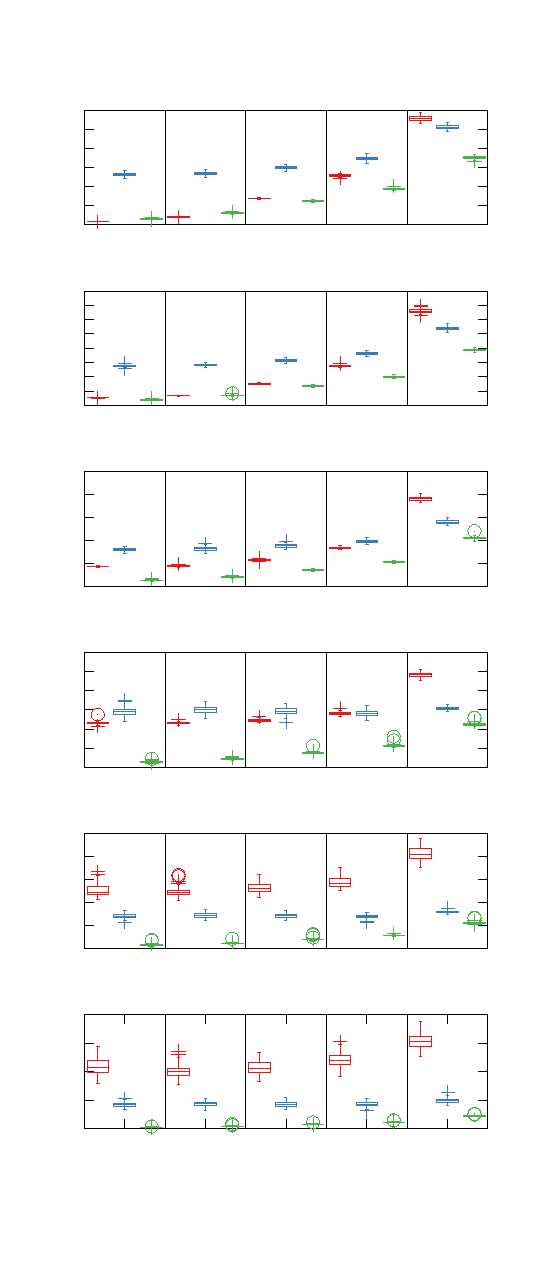
\includegraphics{./figures/experiments/errors_CSM_NDT_implm6_short}}%
    \gplfronttext
  \end{picture}%
\endgroup

  \vspace{-1.5cm}
  \caption{\small Distribution of mean errors of CSM (red), NDT (blue), and
           FSM (our approach) across a range of maximal positional and
           orientational displacements, for progressively larger sensor
           measurement noise levels. The variability of FSM's rigid body
           transformation error is consistent across all configurations. Its
           error is independent of the initial displacement of scans for a
           given level of sensor noise}
  \label{fig:errors_sm}
\end{figure}

At small location and orientation displacements between the two input scans
($\overline{\delta}_{xy} \leq $ 0.05 m,
$\overline{\delta}_\theta \leq 2^\circ$), CSM outperforms NDT and FSM for low
levels of sensor noise ($\sigma_R \leq 0.01$ m). However, as noise increases,
FSM starts exhibiting greater robustness and accuracy than CSM. At greater
location and orientation displacements
($\overline{\delta}_{xy} > 0.05$ m, $\overline{\delta}_\theta > 2^\circ$), FSM
is able to maintain errors equal to or lower than CSM across the entirety of
the spectrum of tested noise levels. Compared to the equally
correspondenceless method of NDT, FSM exhibits greater accuracy across all
tested configurations. The magnitude and variability of FSM's errors for a
given level of sensor noise is independent of the displacement of the two input
scans (fig. \ref{fig:laser_odometry}). The juxtaposition of the three methods'
pose errors at high levels of sensor noise highlight the robustness afforded to
FSM by the Discrete Fourier transform and its properties. With regard to
orientation errors, $71.0\%$-$79.6\%$ of all final orientation errors resulted
under $\gamma / 2^{\nu_{\max}+1} = 0.0011$ rad when $\sigma_R = 0.0$ m. In terms
of execution time, CSM ranged from $4.8$ to $20.5$ ms, NDT from $8.1$ to $19.9$
ms, and FSM from $13.2$ to $16.7$ ms. Therefore FSM's exhibits the least
variability to sensor noise and locational and orientational displacement in
terms of runtime.  The measurement frequency of modern LIDAR sensors ranges
from $12$-$20$ Hz; therefore FSM runs in real time in modern processors.



%%%%%%%%%%%%%%%%%%%%%%%%%%%%%%%%%%%%%%%%%%%%%%%%%%%%%%%%%%%%%%%%%%%%%%%%%%%%%%%%
\section{Conclusions}
  \label{section:finale}
  This paper has presented a scan-matching method for panoramic LIDAR sensors.
The approach rests on properties of the DFT, which afford it increased
robustness and accuracy compared to established scan-matching approaches in the
face of measurement noise exhibited by real-life sensors. The C++ code of the
proposed method, along with the implementation of the conducted experiments is
available at \url{}, .


%%%%%%%%%%%%%%%%%%%%%%%%%%%%%%%%%%%%%%%%%%%%%%%%%%%%%%%%%%%%%%%%%%%%%%%%%%%%%%%%
\newpage
\begin{thebibliography}{99}
  \input{./sections/bibliography.bib}
\end{thebibliography}

%%%%%%%%%%%%%%%%%%%%%%%%%%%%%%%%%%%%%%%%%%%%%%%%%%%%%%%%%%%%%%%%%%%%%%%%%%%%%%%%
% This command serves to balance the column lengths
% on the last page of the document manually. It shortens
% the textheight of the last page by a suitable amount.
% This command does not take effect until the next page
% so it should come on the page before the last. Make
% sure that you do not shorten the textheight too much.
%\addtolength{\textheight}{-1cm}

\balance

\end{document}
